%%%%%%%%%%%%%%%%%%%%%%%%%%%%%%%%%%%%%%%%%%%%%%%%%%
\section{Event Simulation}
%%%%%%%%%%%%%%%%%%%%%%%%%%%%%%%%%%%%%%%%%%%%%%%%%%
Event simulated with the following step
\begin{itemize}
\item Physics process and energy deposition of the beam particles (GEANT3)
\item Conversion of the energy deposition to number of the ionization electrons
\item Drift of the ionization electrons from the point of energy deposition to Anode plane
\item Preamp response, and digitization
\item Noise
\end{itemize}

\subsection{Energy Deposition in TPC}

We use GEANT3 for simulating energy deposition of initial beam particles and
secondary particles to the TPC detector and beam line counters. 
Maximum step of GEANT is set to 0.5 mm which is enough smaller than the TPC readout pitch of 1 cm,
and it means charge deposition in one strip is simulated with more 20 GEANT steps.
We set energy cut-off for soft electron/photon emission to
10 keV which is minimum possible energy can be set in GEANT3.
This cut-off is important for ionization electron recombination.

\subsection{Electric Field}

Figure~\ref{Fit:2DFieldMap} shows electric field of the TPC in V/cm which is calculated using a 2D FEM 
(Finite Element Method) package \cite{Ref:FEMTET},
where horizontal axis, vertical axis, and color strength 
correspond to the beam line direction, the drift direction, the electric field in V/cm, respectively.
Cathode, Anode, and Anode grid are located at of z=-200 mm, z=200 mm, and z=210 mm. respectively.
There are significant distortion of the electric field around 4 corners of the TPC fiducial volume,
and also around x=$\pm$120 mm where support structure of the Cathode and Anode grids exists.

\begin{figure}[htbp]
 \begin{center}
  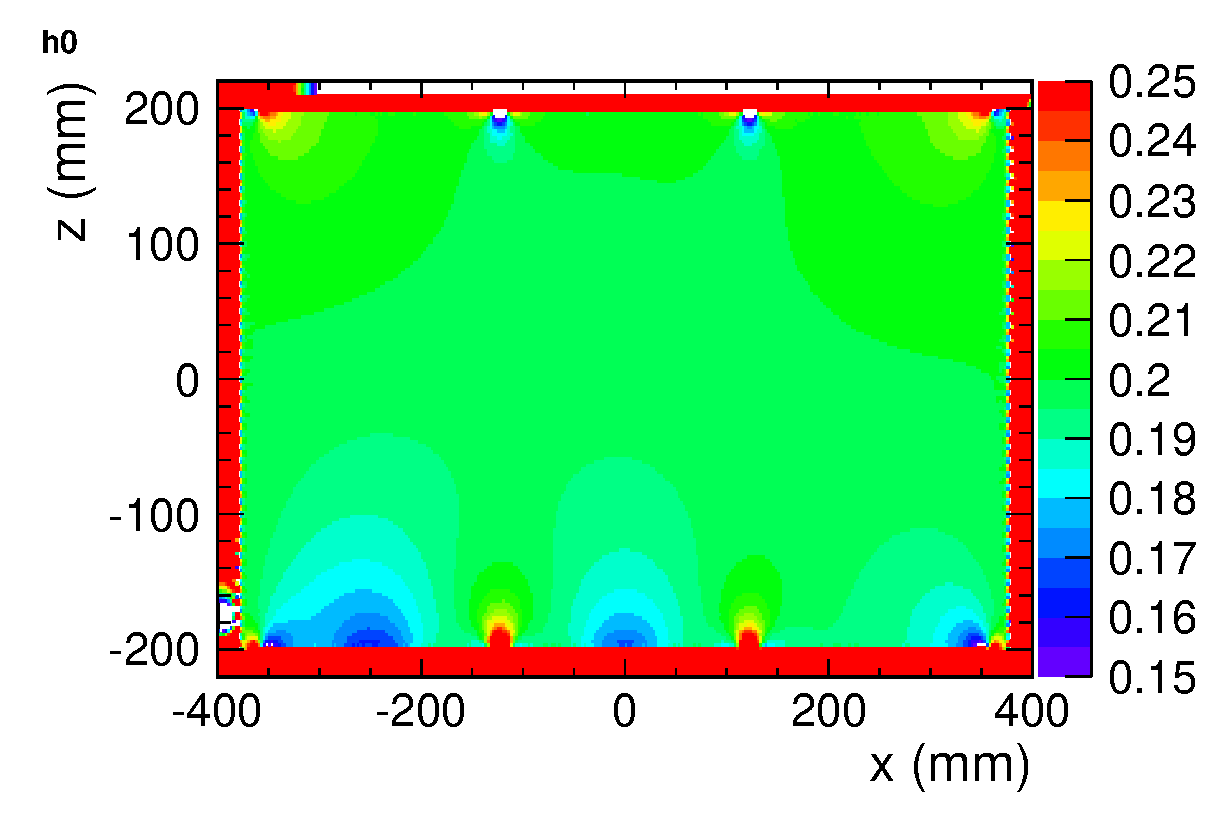
\includegraphics[width=100mm]{fig/2DFieldMap.eps}
 \end{center}
 \caption{Electric field map obtained with 2D FEM where
horizontal axis corresponds to the beam line direction,
and vertical axis corresponds to drift direction,
and color strength corresponds to electric field strength in V/cm.
}
 \label{Fig:2DFieldMap}
\end{figure}

\subsection{Drift Electron Simulation}

Recombination of electron and Argon ion depends on
the electric field $E$ and $dE/dx$,
\begin{equation}
  Q = A\frac{Q_{0}}{1+(k/E)\times(dE/dx)\times(1/\rho)}
\end{equation}
where $Q_{0}$ is initial ionization charge which is obtained from GEANT, $\rho$ is density of liquid Argon (=1.4 g/cm$^3$).
For $A$ and $k$, we use the measurement by ICARUS collaboration \cite{658352}.

After the recombination, drift of the ionization electrons is simulated
using a step simulation with step size of 0.1 mm.
Drift velocity of the ionization electron depends on the liquid Argon temperature
and the electric field. We use a measurement by ICARUS collaboration \cite{649233}.
Typical drift velocity with 200 V/cm of the drift field and temperature of 92K is 0.8 m/ms.
Diffusion of the drift electron is considered and we assume size of the transverse diffusion and and lateral diffusion
are 3.0 mm/m and 1.5 mm/m, respectively.
Figure~\ref{Fig:DriftSimulation} shows simulated track of the drift electrons with three different positions.
left plot with x= 0 mm corresponds to the center of the TPC detector, 
middle plot with x= 130 mm corresponds to the location of anode grid frame,
and right plot with x= 350 mm corresponds to the edge of the TPC fiducial.
Because of the field distortion we find significant displacement of the drift electron in
x direction for x=130 and x=350. It is a main source of the non-uniformity observed in 
the through-going pion response (Fig.~\ref{fig:PionQvsCh}).

\begin{figure}[htbp]
 \begin{center}
  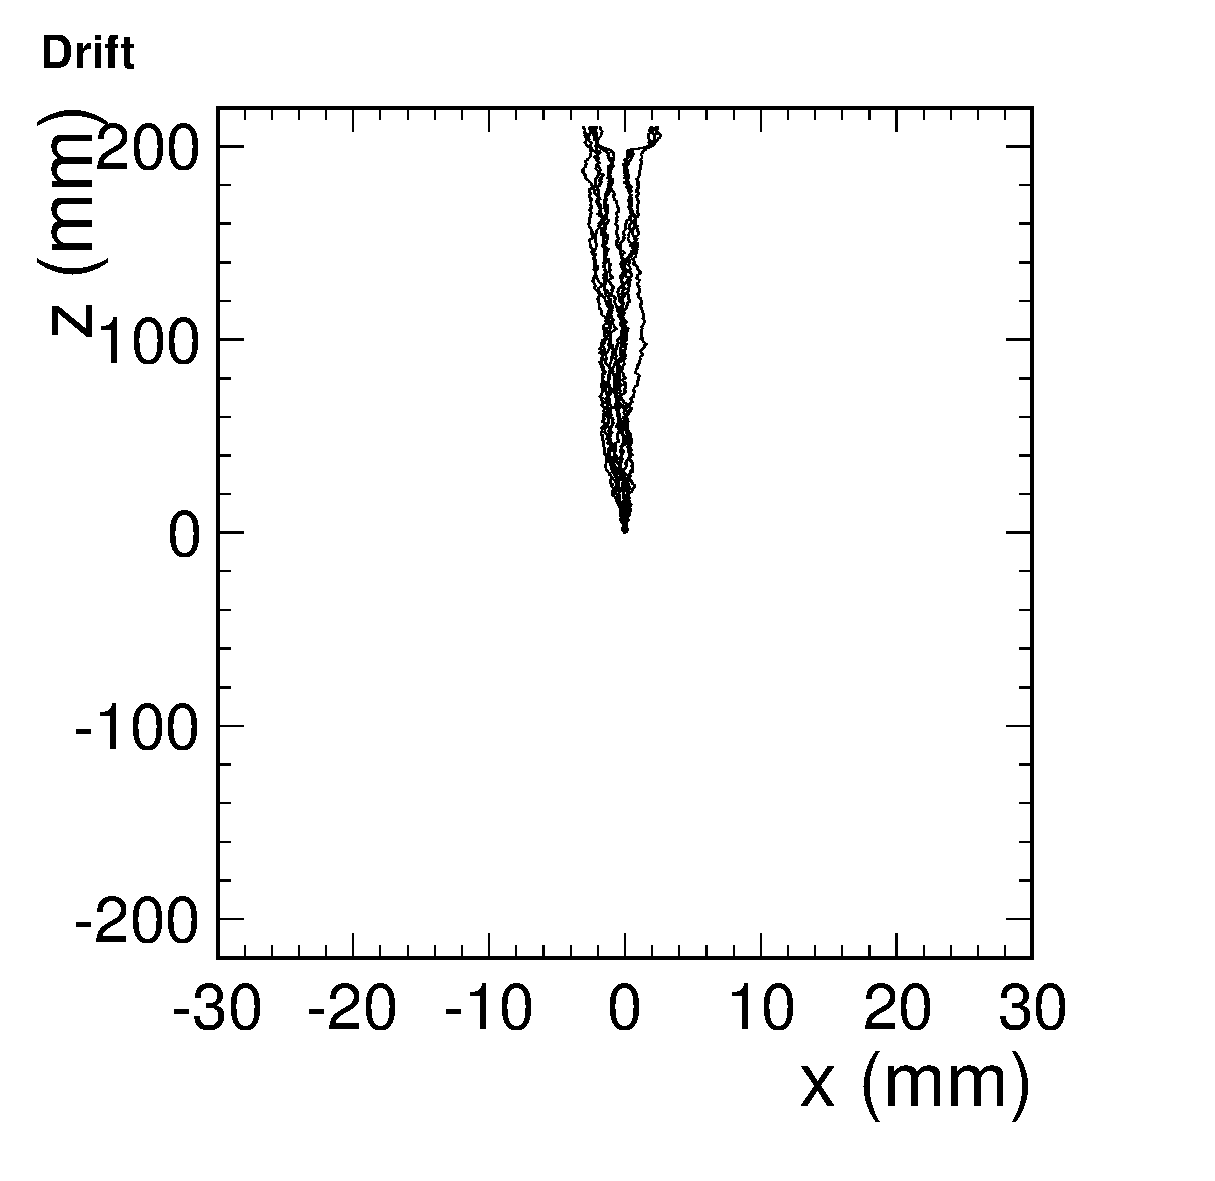
\includegraphics[width=40mm]{fig/Drift_0.eps}
  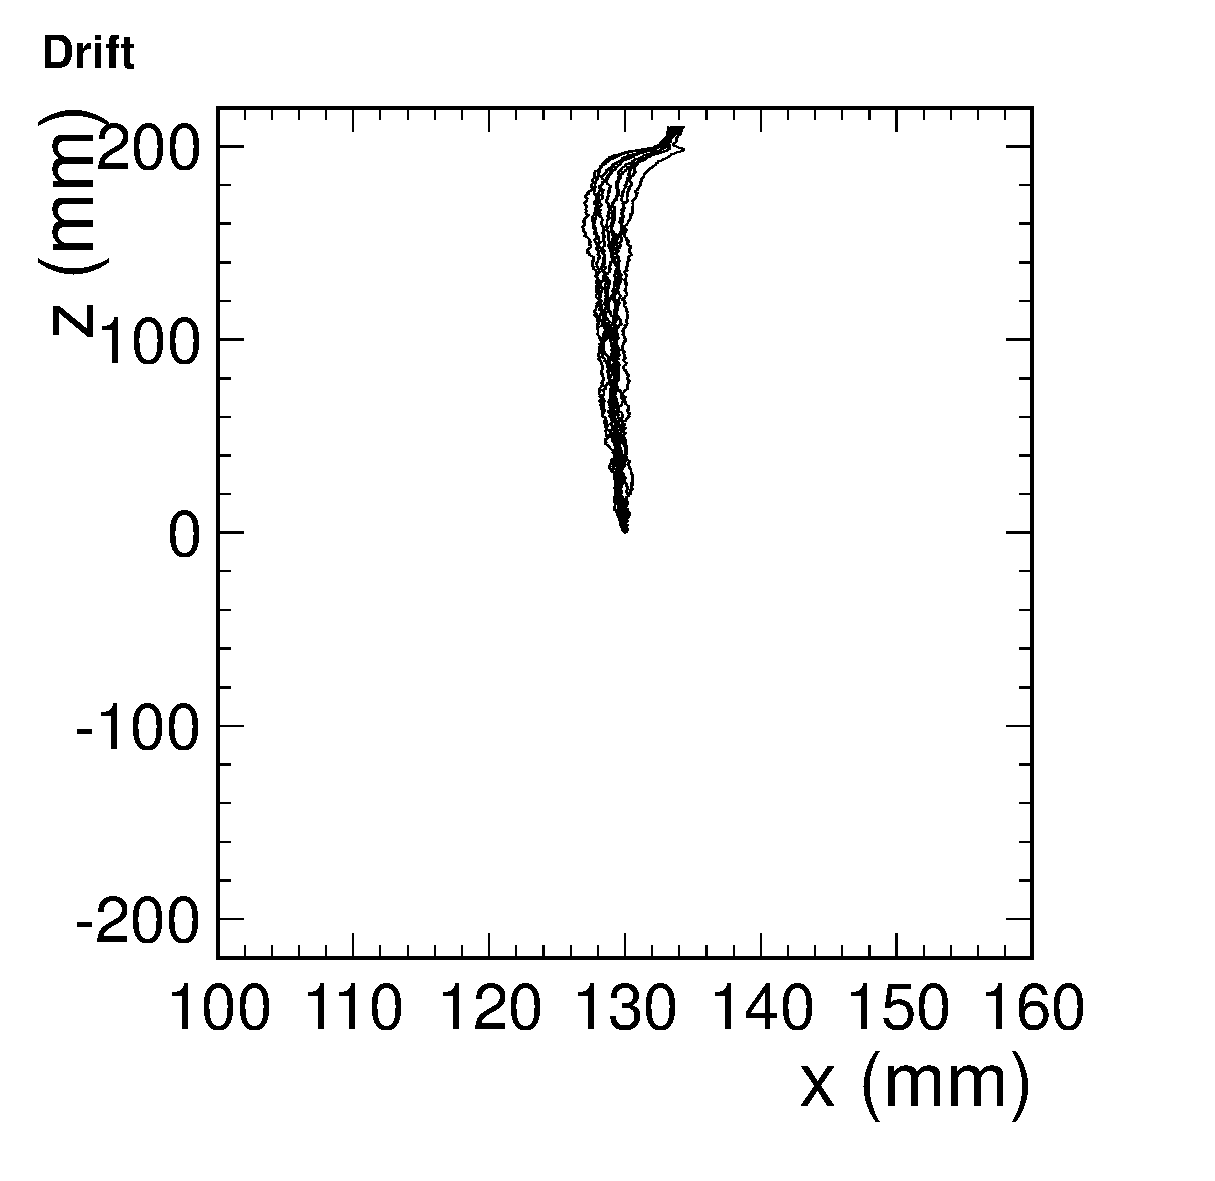
\includegraphics[width=40mm]{fig/Drift_130.eps}
  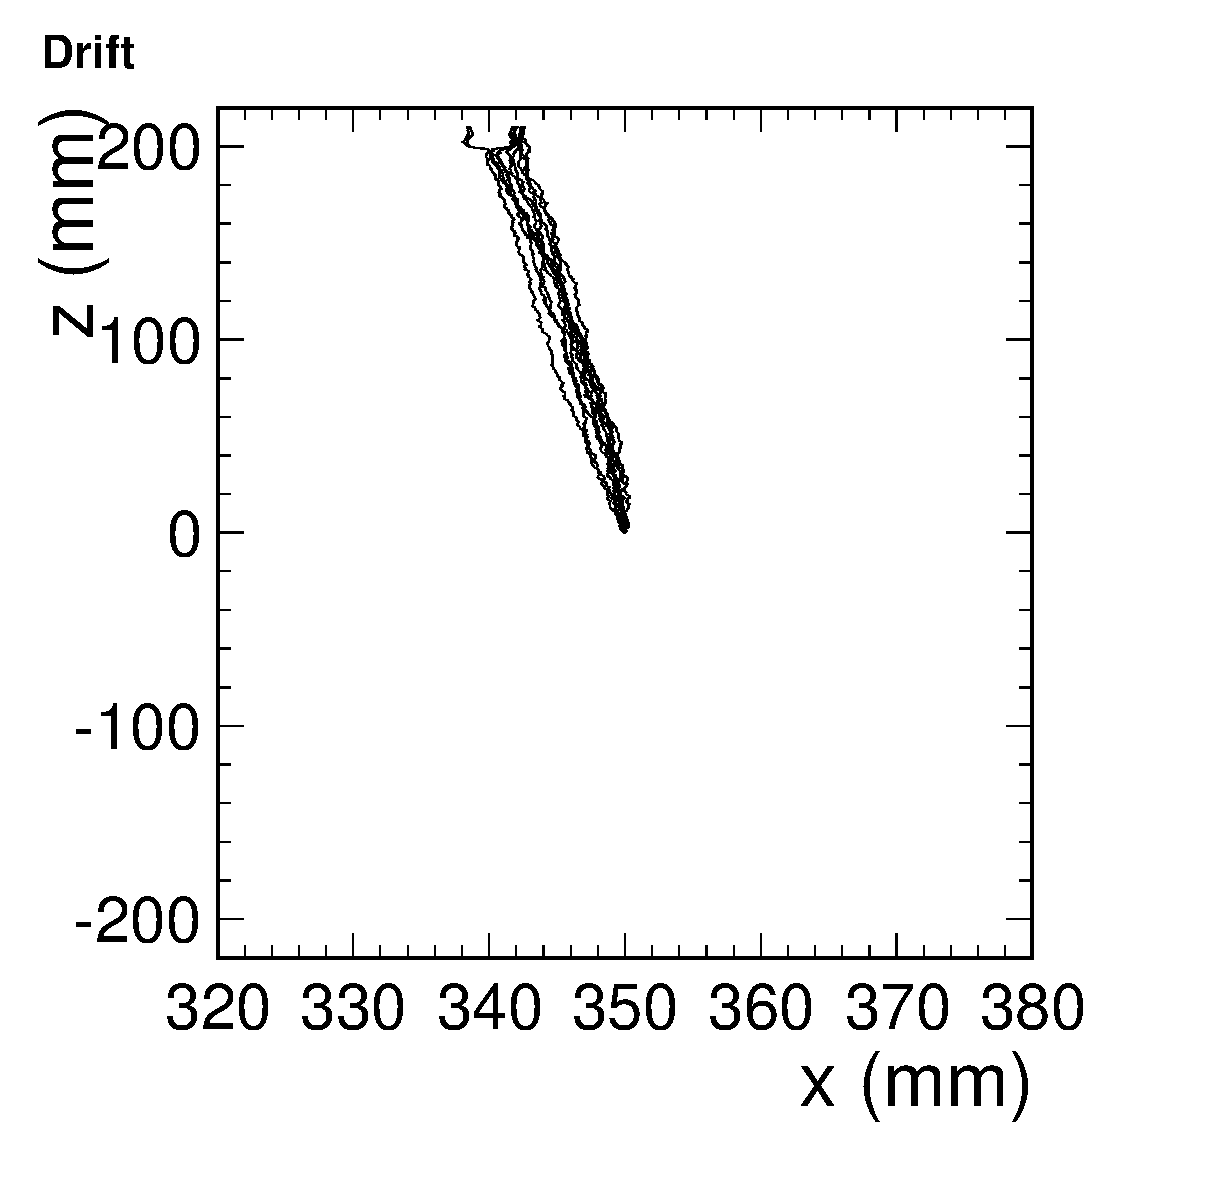
\includegraphics[width=40mm]{fig/Drift_350.eps}
 \end{center}
 \caption{Simulation of the electron drift with three different positions of energy deposition. Left, middle, and right plots corresponds to x=0, x=130 mm, and x=350 mm, respectively.}
 \label{Fig:DriftSimulation}
\end{figure}

%\begin{itemize}
%\item Plot: drift simulation  (Tanaka)
%\end{itemize}


\subsection{Preamp Response and Digitization}
%\begin{itemize}
%\item Preamp gain vs channel number  (Naito)
%\end{itemize}

%\subsection{FFT Noise}
\subsection{FFT Noise}
There are two kinds of noise in the data we obtained, random noise and coherent noise.
Random noise is the noise which exists in each anode channel.
Coherent noise is in each board.
The pseudo noise we implemented in Monte Carlo simulation is composed of random and coherent noise by this reason.

Random noise is generated from FFT(Fast Fourier Transform) distribution of real data. Figure \ref{example10ch} shows an example of FFT distribution.

Coherent noise is generated board by board as the noise scale in the real data we obtained.
The noise scale is defined as a root mean square of pedestal, minimum noise scale is about 3 and maximum noise scale is about 10 in the data.

The ratio of random and coherent noise is 1:1 as equation \ref{PseudoNoise}.
Figure \ref{DATAnoise} shows real data noise and Fig.\ref{MCnoise} shows pseudo noise we implemented in Monte Carlo simulation.
\begin{equation}
  Pseudo\,Noise = \frac{Random\,Noise + Coherent\,Noise}{2}
  \label{PseudoNoise}
\end{equation}

\begin{figure}[!htb]
  \centering
  \centering
  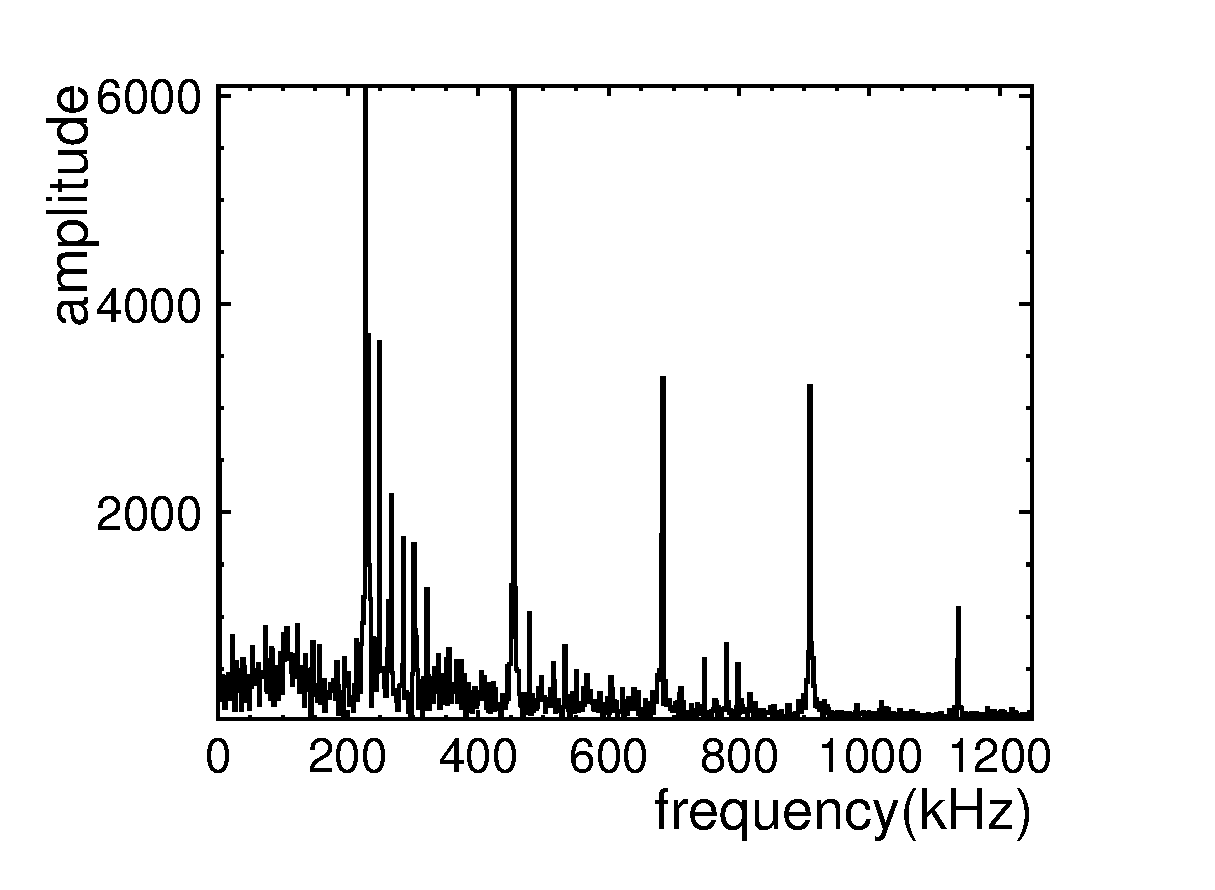
\includegraphics[width=10cm,clip]{./fig/FFTdist.eps}
  \caption{An example distribution of frequency}
  \label{example10ch}
\end{figure}
%\begin{figure}[!htb]
%  \centering
%  \centering
%  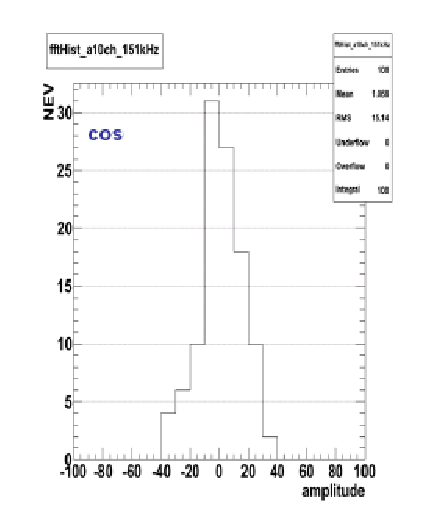
\includegraphics[width=11cm,clip]{./fig/cos.eps}
%  \caption{An example of distribution of amplitude}
%  \label{ampDist}
%\end{figure}
%\begin{figure}[!htb]
%  \centering
%  \centering
%  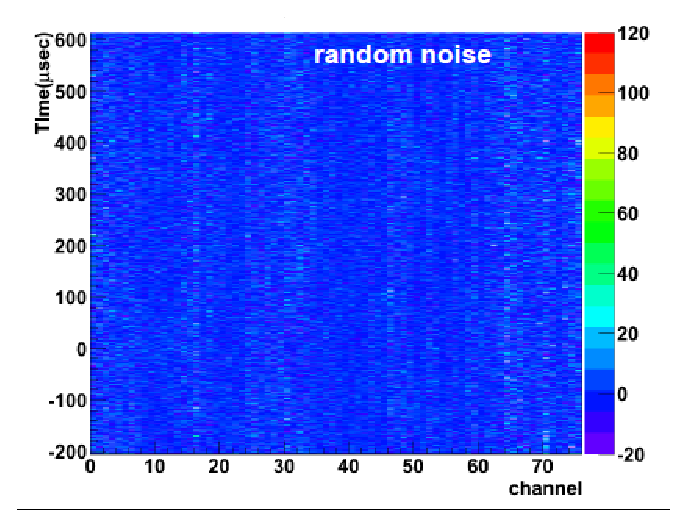
\includegraphics[width=11cm,clip]{./fig/randomnoise.eps}
%  \caption{Random noise}
%  \label{randomNoise}
%\end{figure}
\begin{figure}[!htb]
\begin{minipage}{0.5\hsize}
  \centering
  \includegraphics[width=7cm,clip]{./fig/DATAnoise.eps}
  \caption{Data noise}
  \label{DATAnoise}
\end{minipage}
\begin{minipage}{0.5\hsize}
  \centering
  \includegraphics[width=7cm,clip]{./fig/MCnoise.eps}
  \caption{Pseudo noise(Noise simulation)}
  \label{MCnoise}
\end{minipage}
\end{figure}
%\begin{figure}[!htb]
%  \centering
%  \centering
%  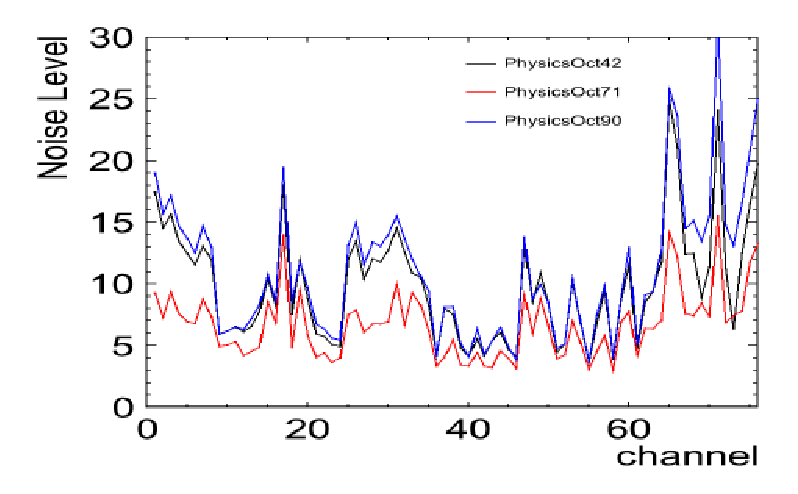
\includegraphics[width=11cm,clip]{./fig/scaling.eps}
%  \caption{Noise level}
%  \label{scaling}
%\end{figure}

%\subsection{Cross Talk}
\subsection{Cross Talk}

The distance between anode channels is very short,
so the influence of mutual capacitance become large
and this capacitive coupling induce cross talk noise.
This effect notably appears the channel where the differnce of the charge between adjacents channels is large, such as the channel around stopped point of proton.
Figure\ref{fig:cross_talk1} shows the signal wave form of stopped channel and the front channel of typical proton event.
The signal wave form of stopped channel is differencial form of the one of the front channel.
This shape is appeared at channel number 1 which cannot enter drifted ionization electron in electric power lines.
These facts show the exisitence of cross talk.
Then, we implement this crosstalk phenomenon in Monte Carlo Simulation
by adding bipolar shape of the signal gaussian shape at adjacent channels.
The area of the mountain of cross talk bipolar shape is 10.5\% of the area of signal gaussian at each adjacent channel.
The value of 10.5\% is determined by comparing the distribuntion of integrated ADC at stopped channel between DATA and MC.
Figure\ref{fig:cross_talk2} shows integrated ADC distribution of stopped channel.
Black is DATA and blue is simulation with cross talk red is simulation without cross talk.
As this figure shows, DATA and MC with cross talk is good agreement,
and the value of 10.5\% is reasonable.

\begin{figure}[htbp]
  \begin{tabular}{cc}
    \begin{minipage}{0.5\hsize}
      \centering
      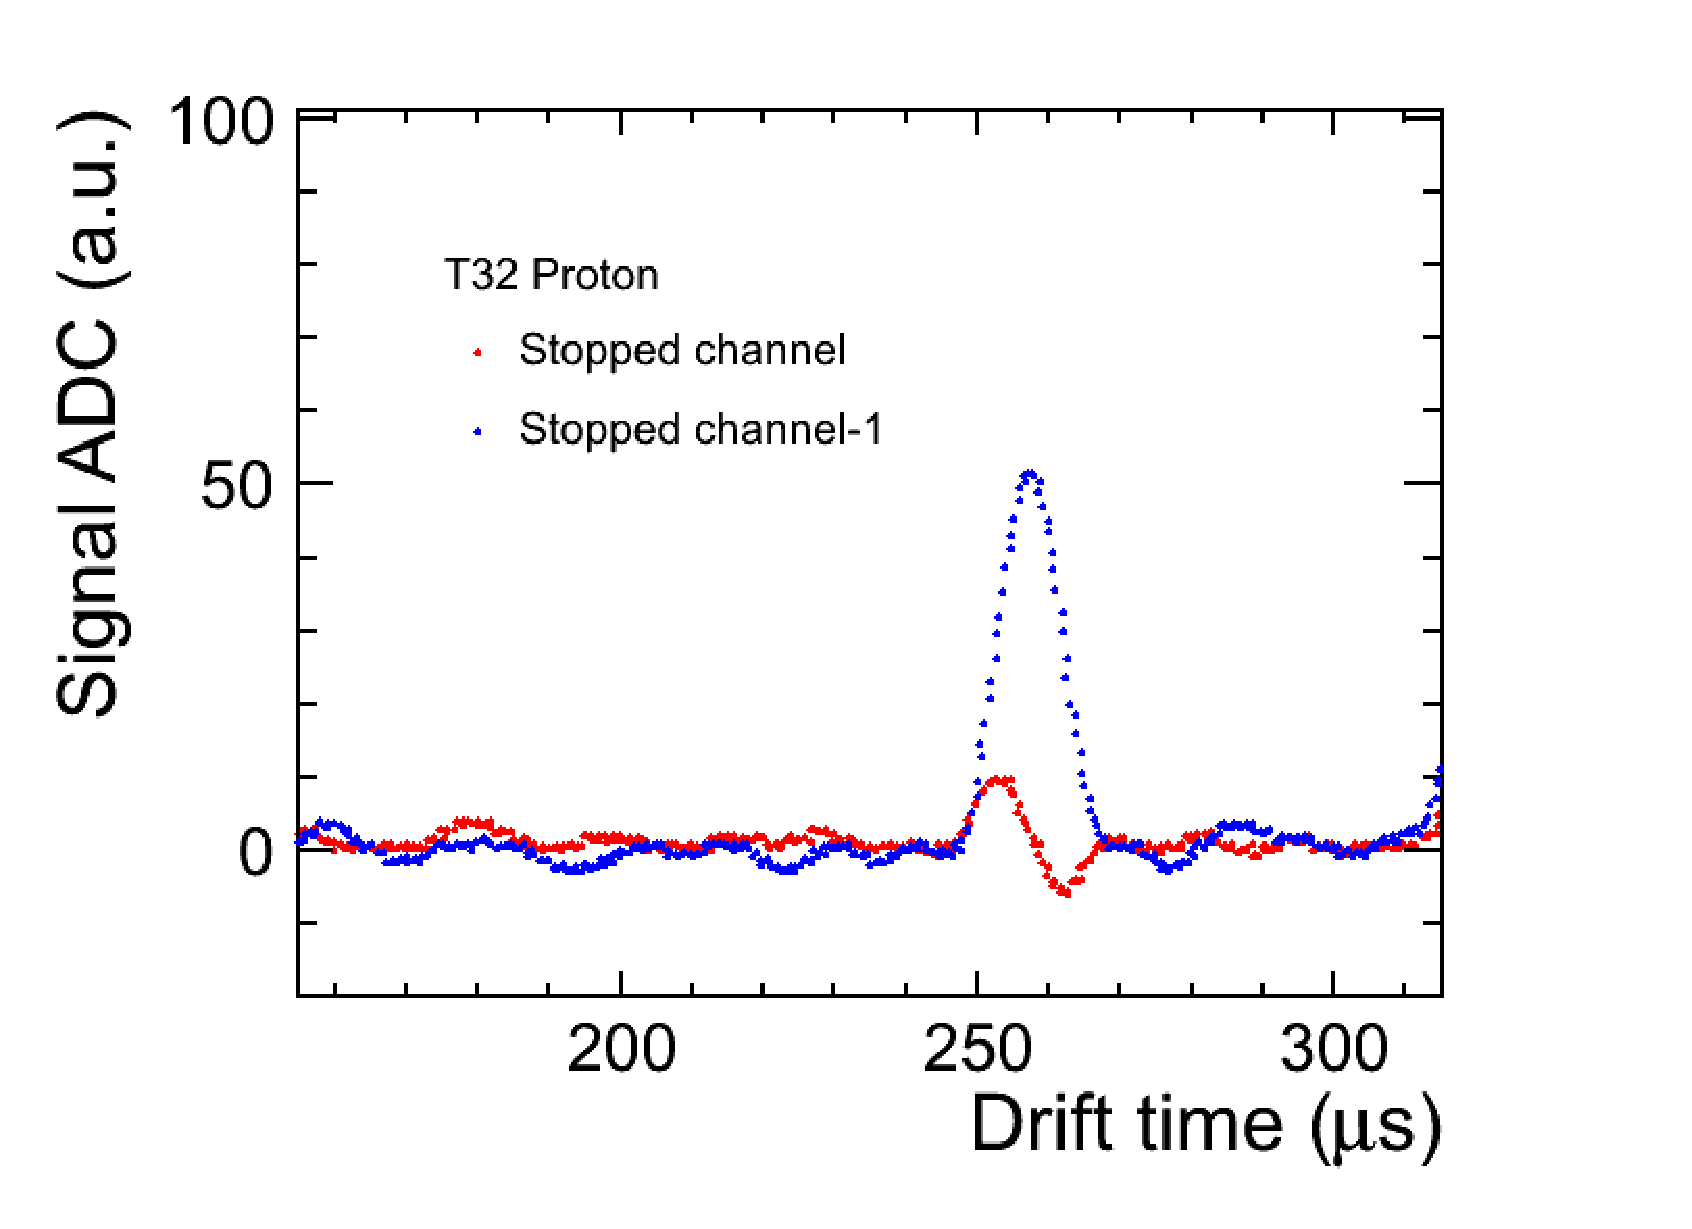
\includegraphics[width=6cm,clip]{fig/cross_talk_1.eps}
      \caption{Signal wave form of stopped channel and the front channel}
      \label{fig:cross_talk1}
    \end{minipage}
    \begin{minipage}{0.5\hsize}
      \centering
      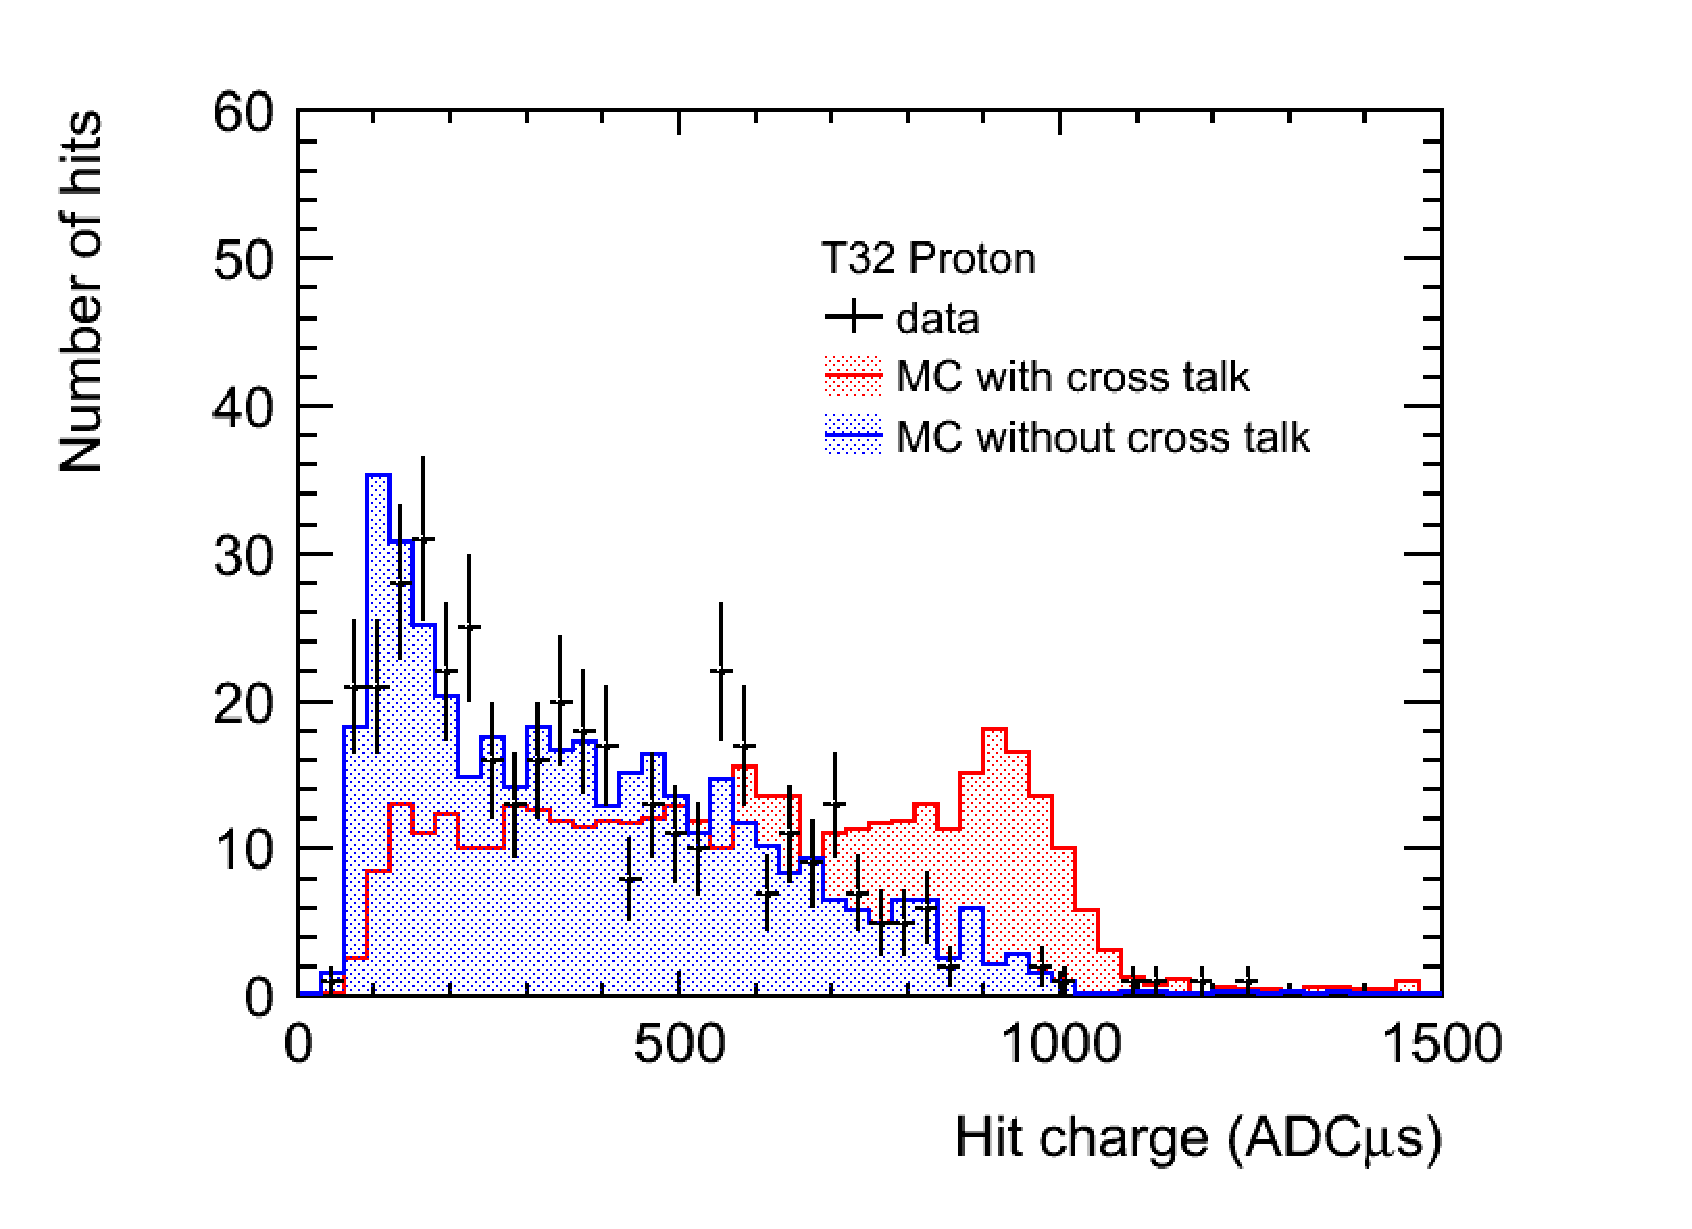
\includegraphics[width=6cm,clip]{fig/cross_talk_2.eps}
      \caption{Integrated ADC distribution of stopped channel}
      \label{fig:cross_talk2}
    \end{minipage}
  \end{tabular}
\end{figure}




\subsection{Signal and Noise Scale Tuning}
\begin{itemize}
\item Plot: Landau distribution after the tuning  (Tanaka)
\end{itemize}

\subsection{Beam energy}
We estimated a beam momentum using simple MC simulation.
Figure \ref{K11Br_Beam_line} shows MC simulation's geometry.
We generate 800MeV/$c$ pencil beam and shoot the beam downstream.
Figure \ref{k_pi_momentum} shows Kaon and Pion momentum distribution
using this MC simulation at BDC.
Kaon beam momentum is estimated by the momentum distribution of MC simulation.
%Actually, kaon momentum distribution peak is adjusted so that kaon decay point of MC simulation is consistent with data.
%Section \ref{kaon_energy_section} explains this point.
%And proton momentum is estimated in other way, using TREK detector TOF information.
%Section \ref{proton_energy_section} shows proton momentum distribution.

\begin{figure}[!htb]
  \centering
  \centering
  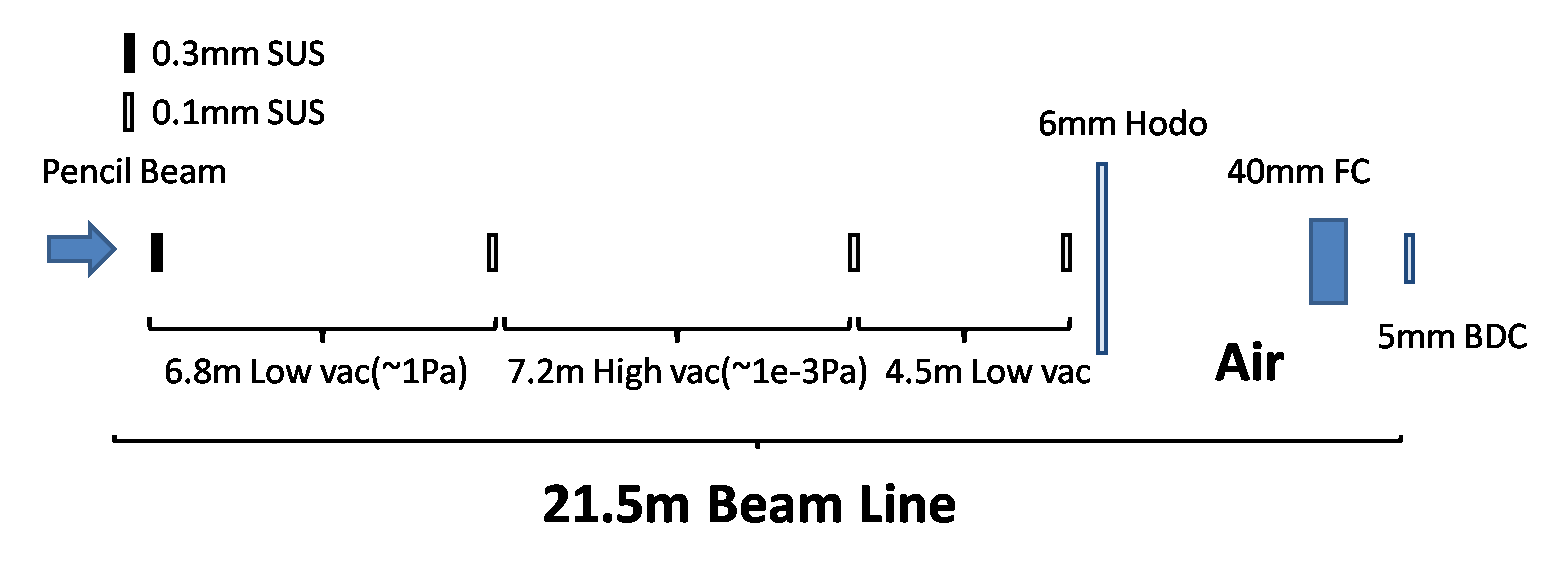
\includegraphics[width=10cm,clip]{./fig/K11Br_beamline_sim.eps}
  \caption{K1.1 Br beam line}
  \label{K11Br_Beam_line}
\end{figure}


\begin{figure}[!htb]
  \centering
  \centering
  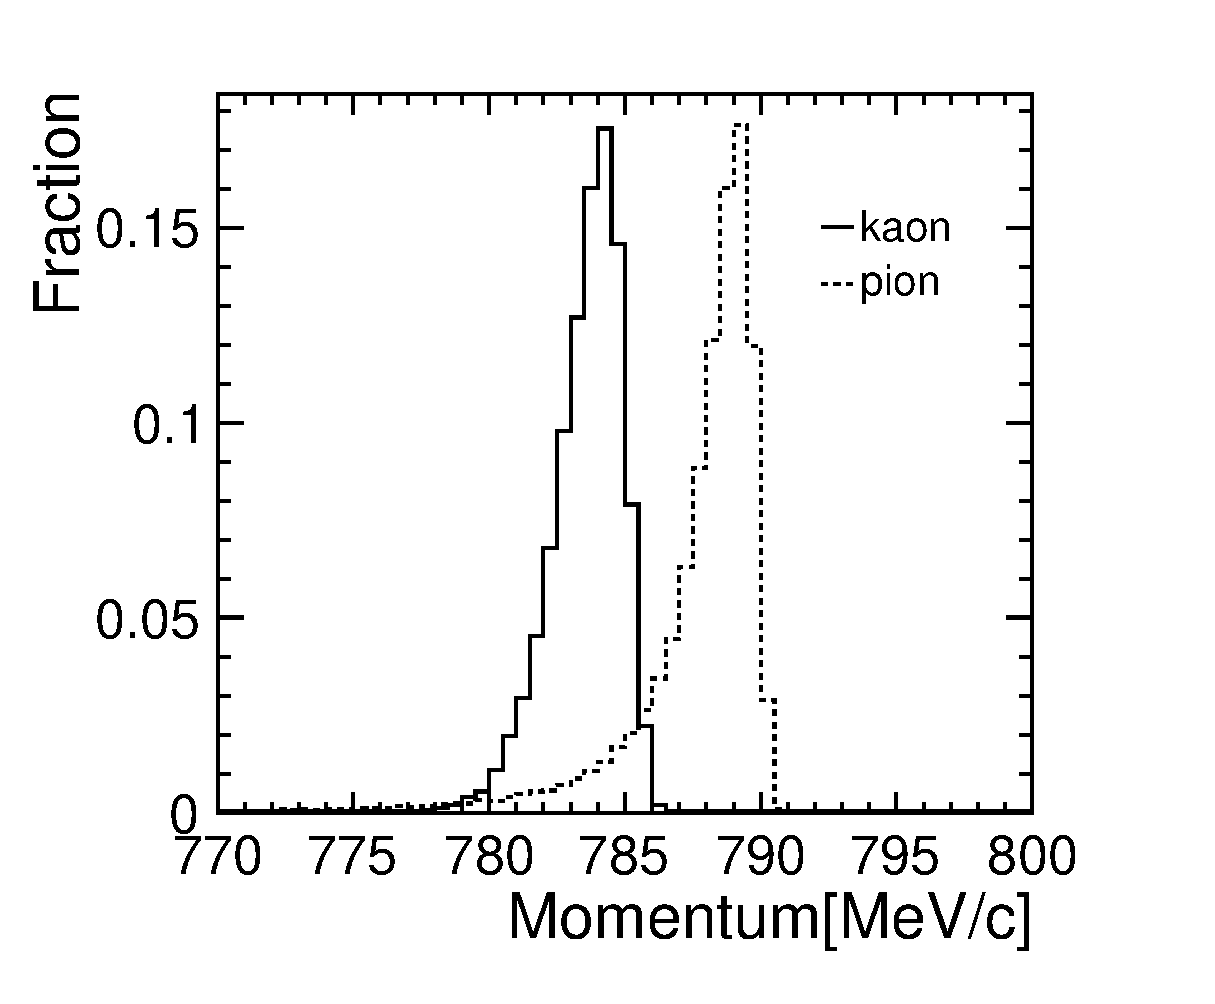
\includegraphics[width=10cm,clip]{./fig/Kaon_pion_momentum_nogrid.eps}
  \caption{Kaon and Pion momentum distribution at BDC}
  \label{k_pi_momentum}
\end{figure}


\subsubsection{Kaon energy
  \label{KaonEnergy}
}
Kaon beam momentum is estimated by the momentum distribution of MC simulation.
We change Kaon beam momentum in a range of 700 - 800 MeV/$c$ and search the momentum that decay point distribution of MC simulation is consistent with data one.

\subsubsection{Proton energy}
Proton momentum shown in Figure \ref{fig:Proton_momentum} is used as proton beam momentum of MC simulation.

\subsubsection{Energy deposition in degrader}
It is too high energy that Kaon beam stops in the fiducial volume of 250LAr TPC.
In order to degrade the beam momentum, some lead glass blocks and a lead brick were inserted in front of 250LAr TPC as degrader.
%We estimate energy deposition in degrader by using MC simulation.
Figure \ref{energy_deposition} shows energy deposition distribution in degrader.


\begin{figure}[!htb]
  \centering
  \centering
  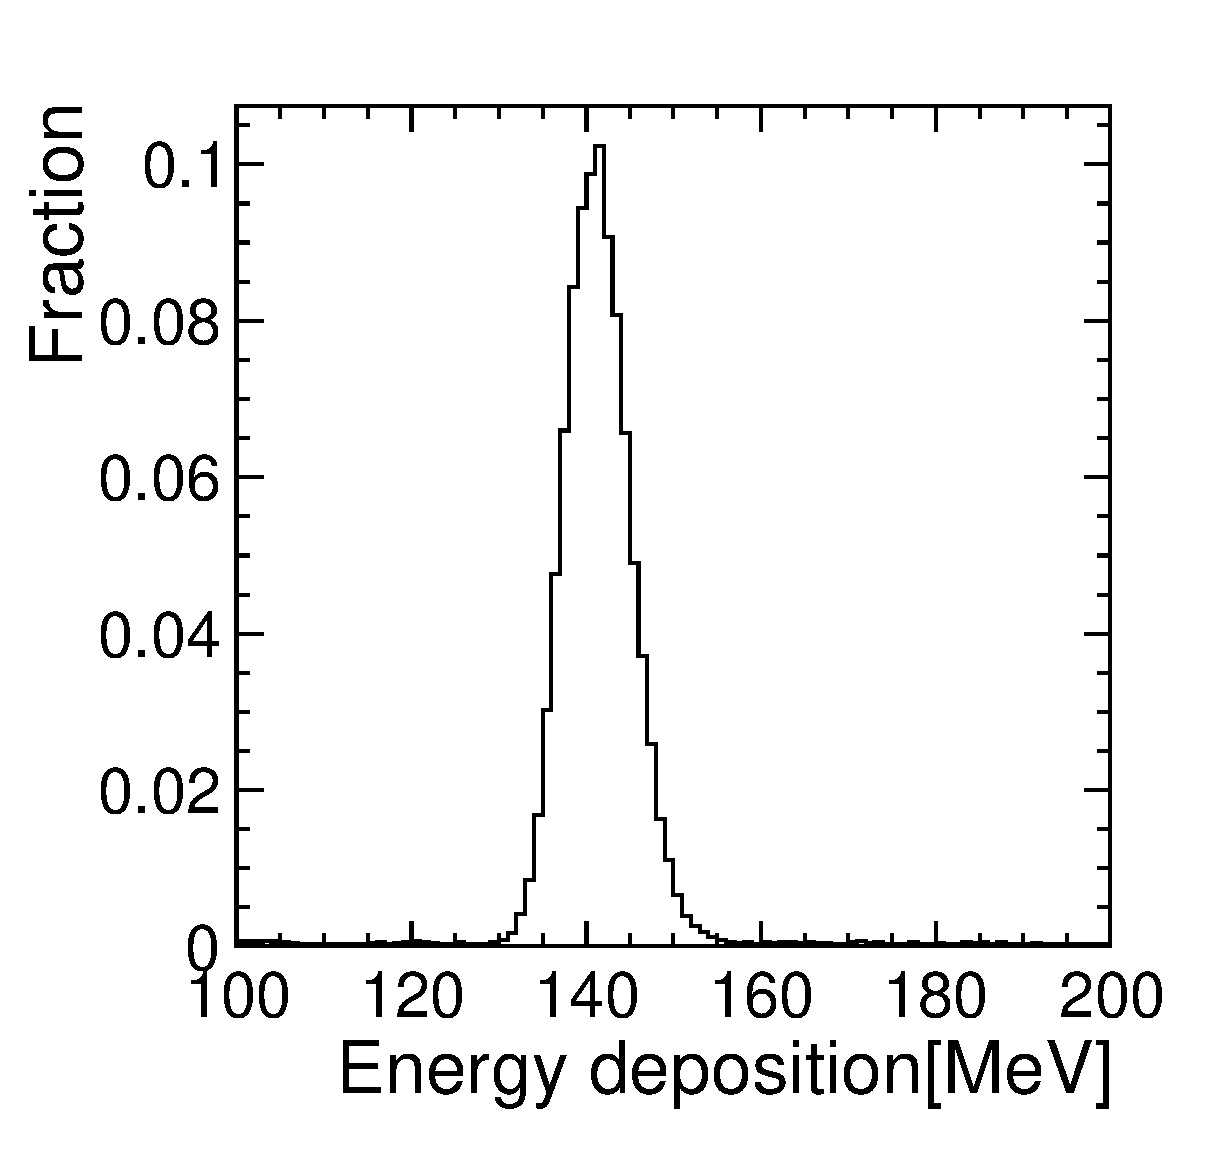
\includegraphics[width=10cm,clip]{./fig/energy_deposition.eps}
  \caption{Energy deposition in degrader}
  \label{energy_deposition}
\end{figure}





